\documentclass{a0poster}
\usepackage{fancytikzposter} % here most of the things are defined
% change parameters only after this line
\usepackage[margin=\margin cm, paperwidth=84.1cm, paperheight=118.9cm]{ geometry}
\title{PISA 2012 - An Interesting Story}
\author{Marcin Kosiński, Norbert Ryciak, Marta Sommer \\Faculty of Mathematics and Information Sciences on Warsaw University of Technology\\\texttt{m.p.kosinski@gmail.com, norbertryciak@gmail.com, mmartasommer@gmail.com}}
\begin{document}
%\AddToShipoutPicture{\BackgroundPicture}
\noindent
\begin{tikzpicture}
\initializesizeandshifts
\titleblock{50}{1}
\blocknode{Studying Mathematics Is Important}{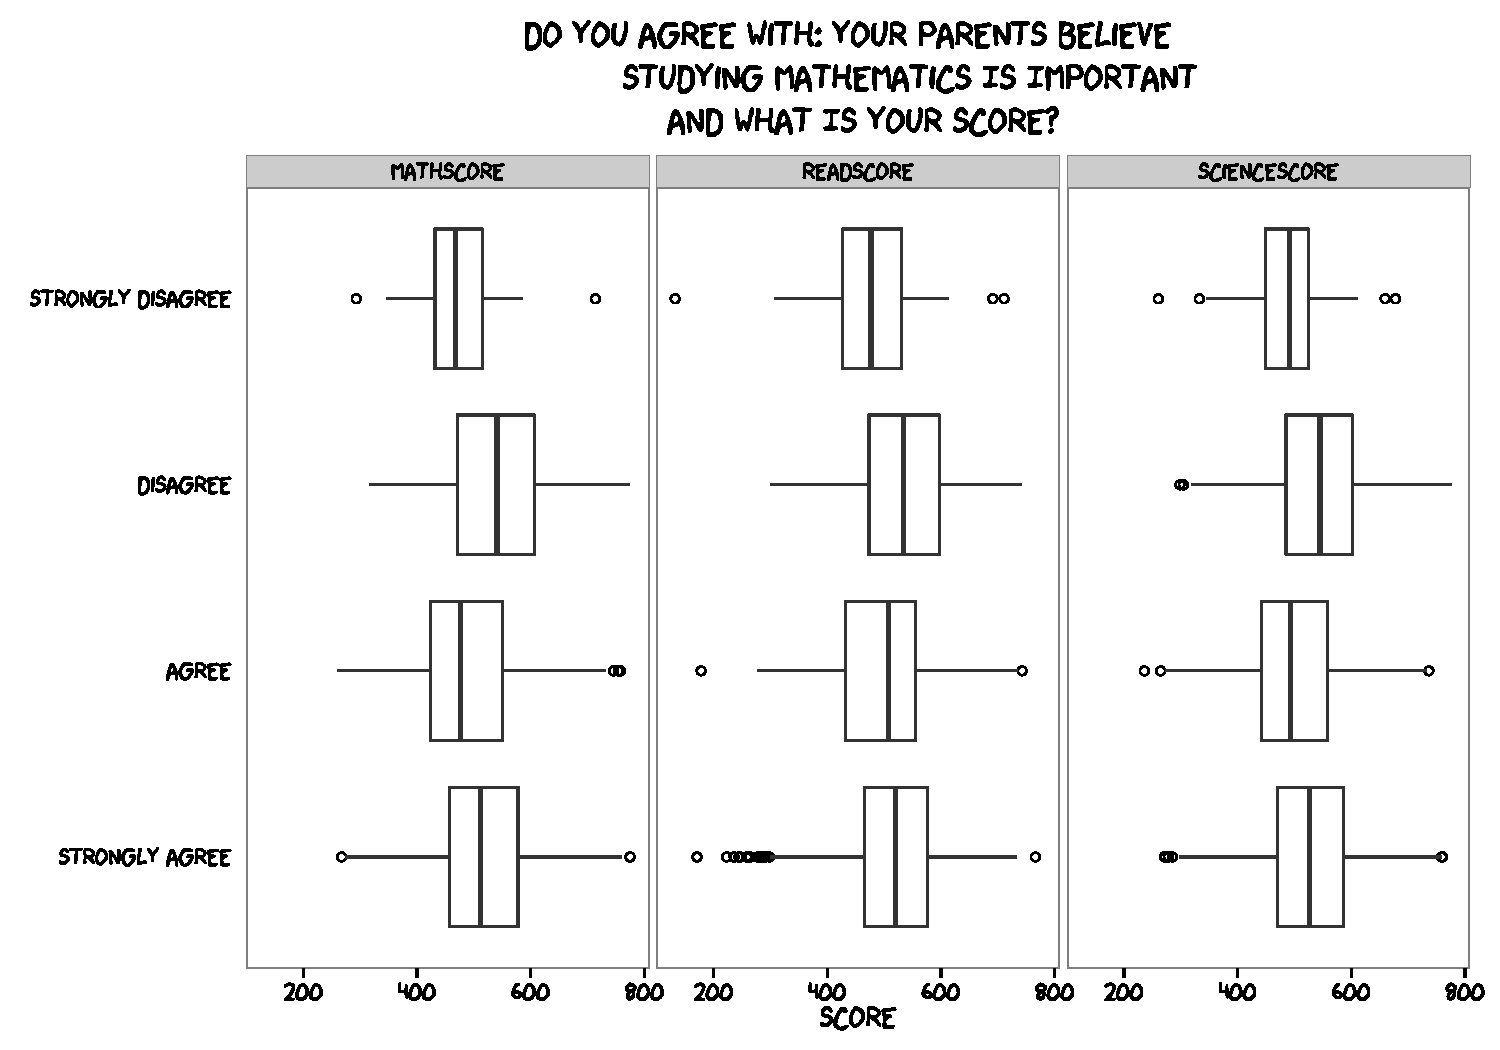
\includegraphics[width=0.9\textwidth]{graphs/Marcin22.pdf}}
\blocknode{I Make Friends Easily}{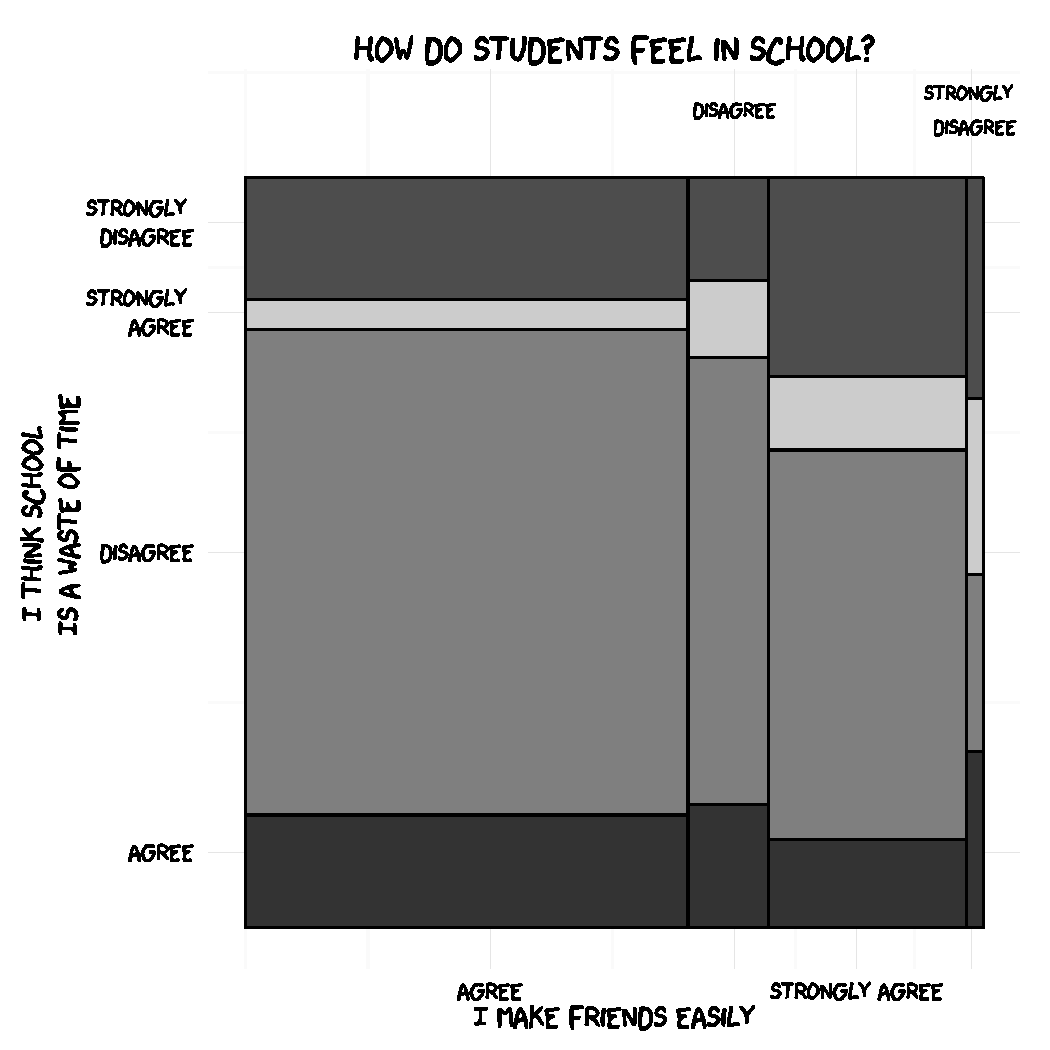
\includegraphics[width=0.9\textwidth]{graphs/Marcin11.pdf}}
\blocknode{Maths Behaviour and Anxiety}{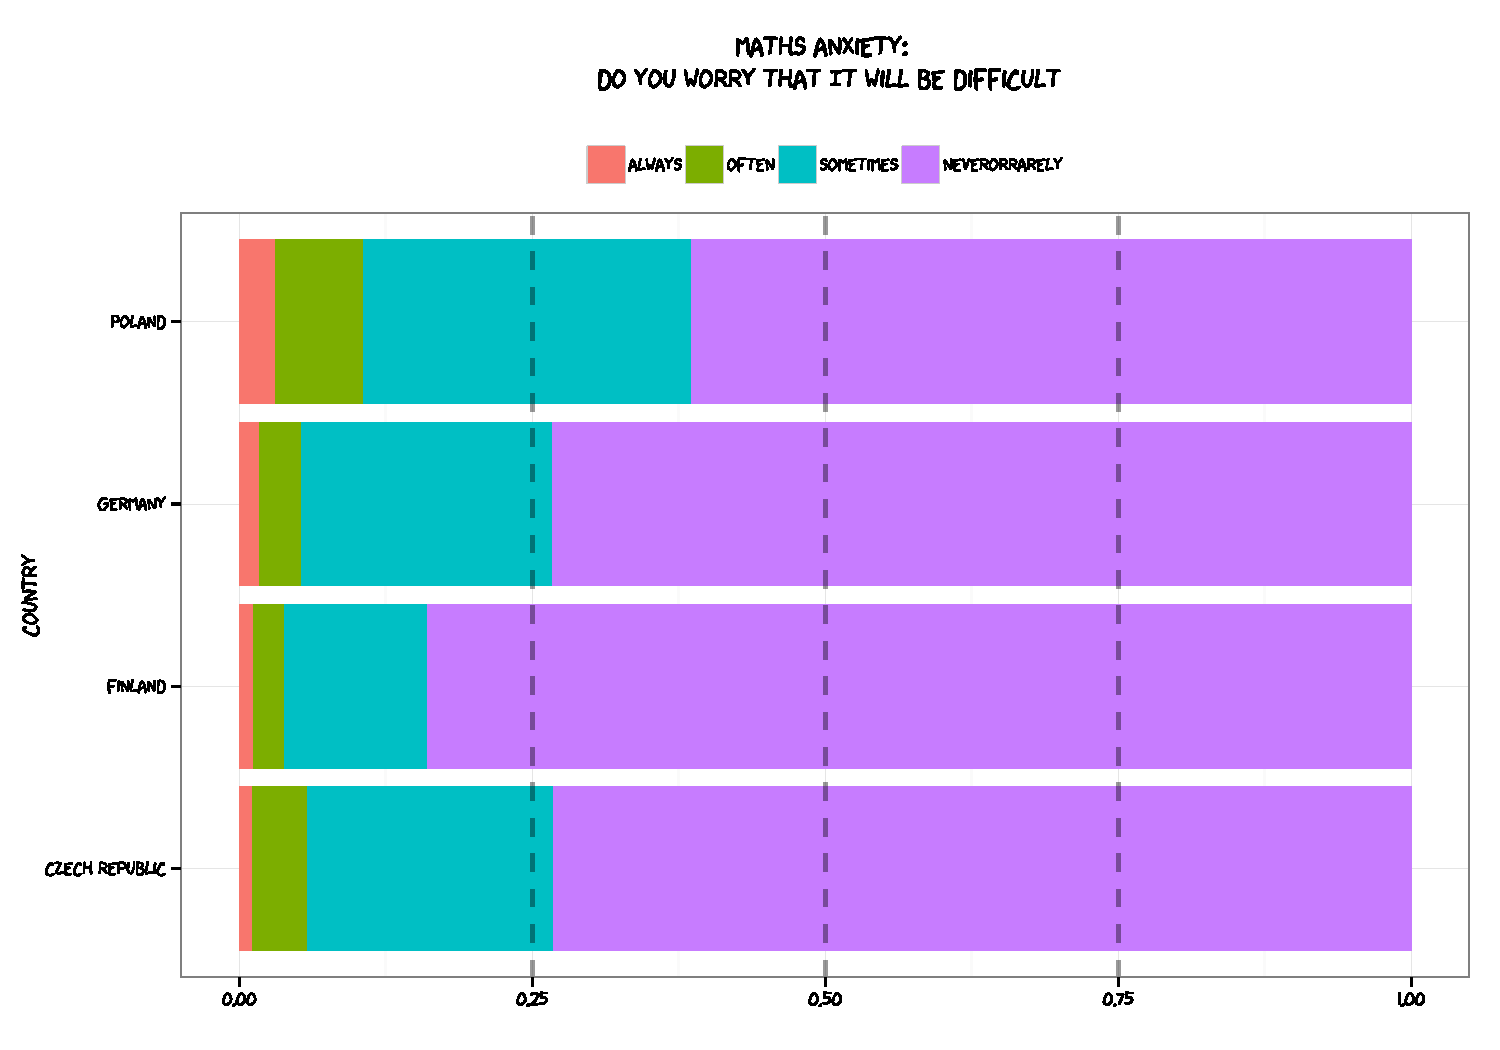
\includegraphics[width=0.9\textwidth, height=12cm]{graphs/Marcin33.pdf}
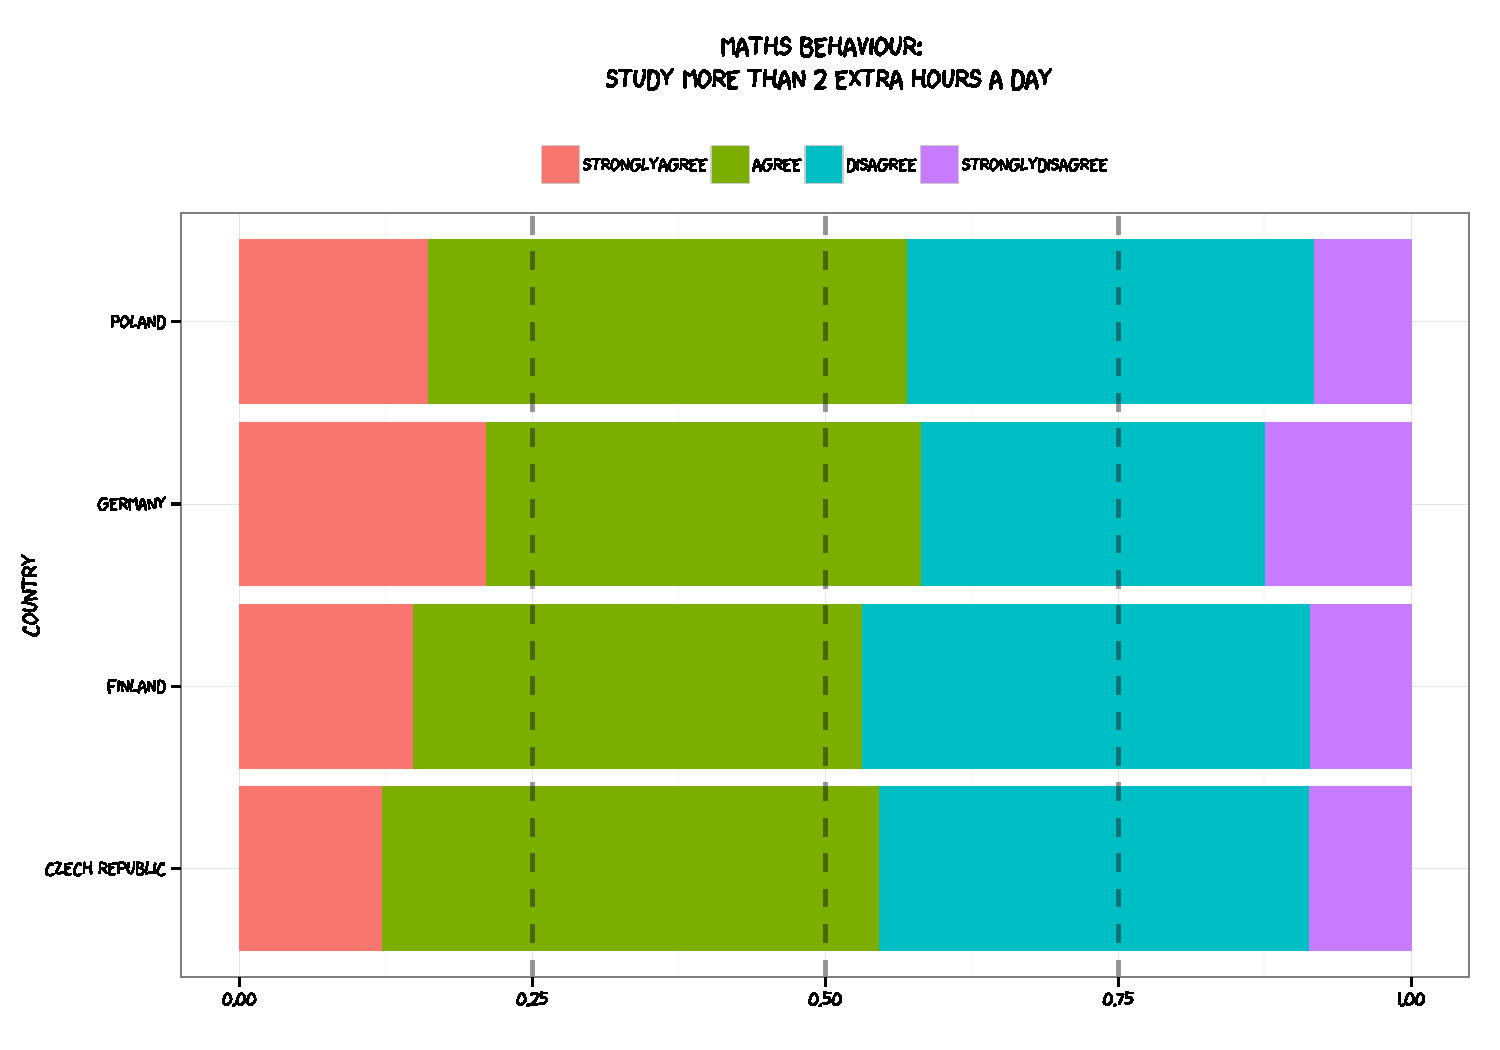
\includegraphics[width=0.9\textwidth, height=12cm]{graphs/Marcin44.pdf}}

\startsecondcolumn
\blocknode{What Is Your Mother Currently Doing?}{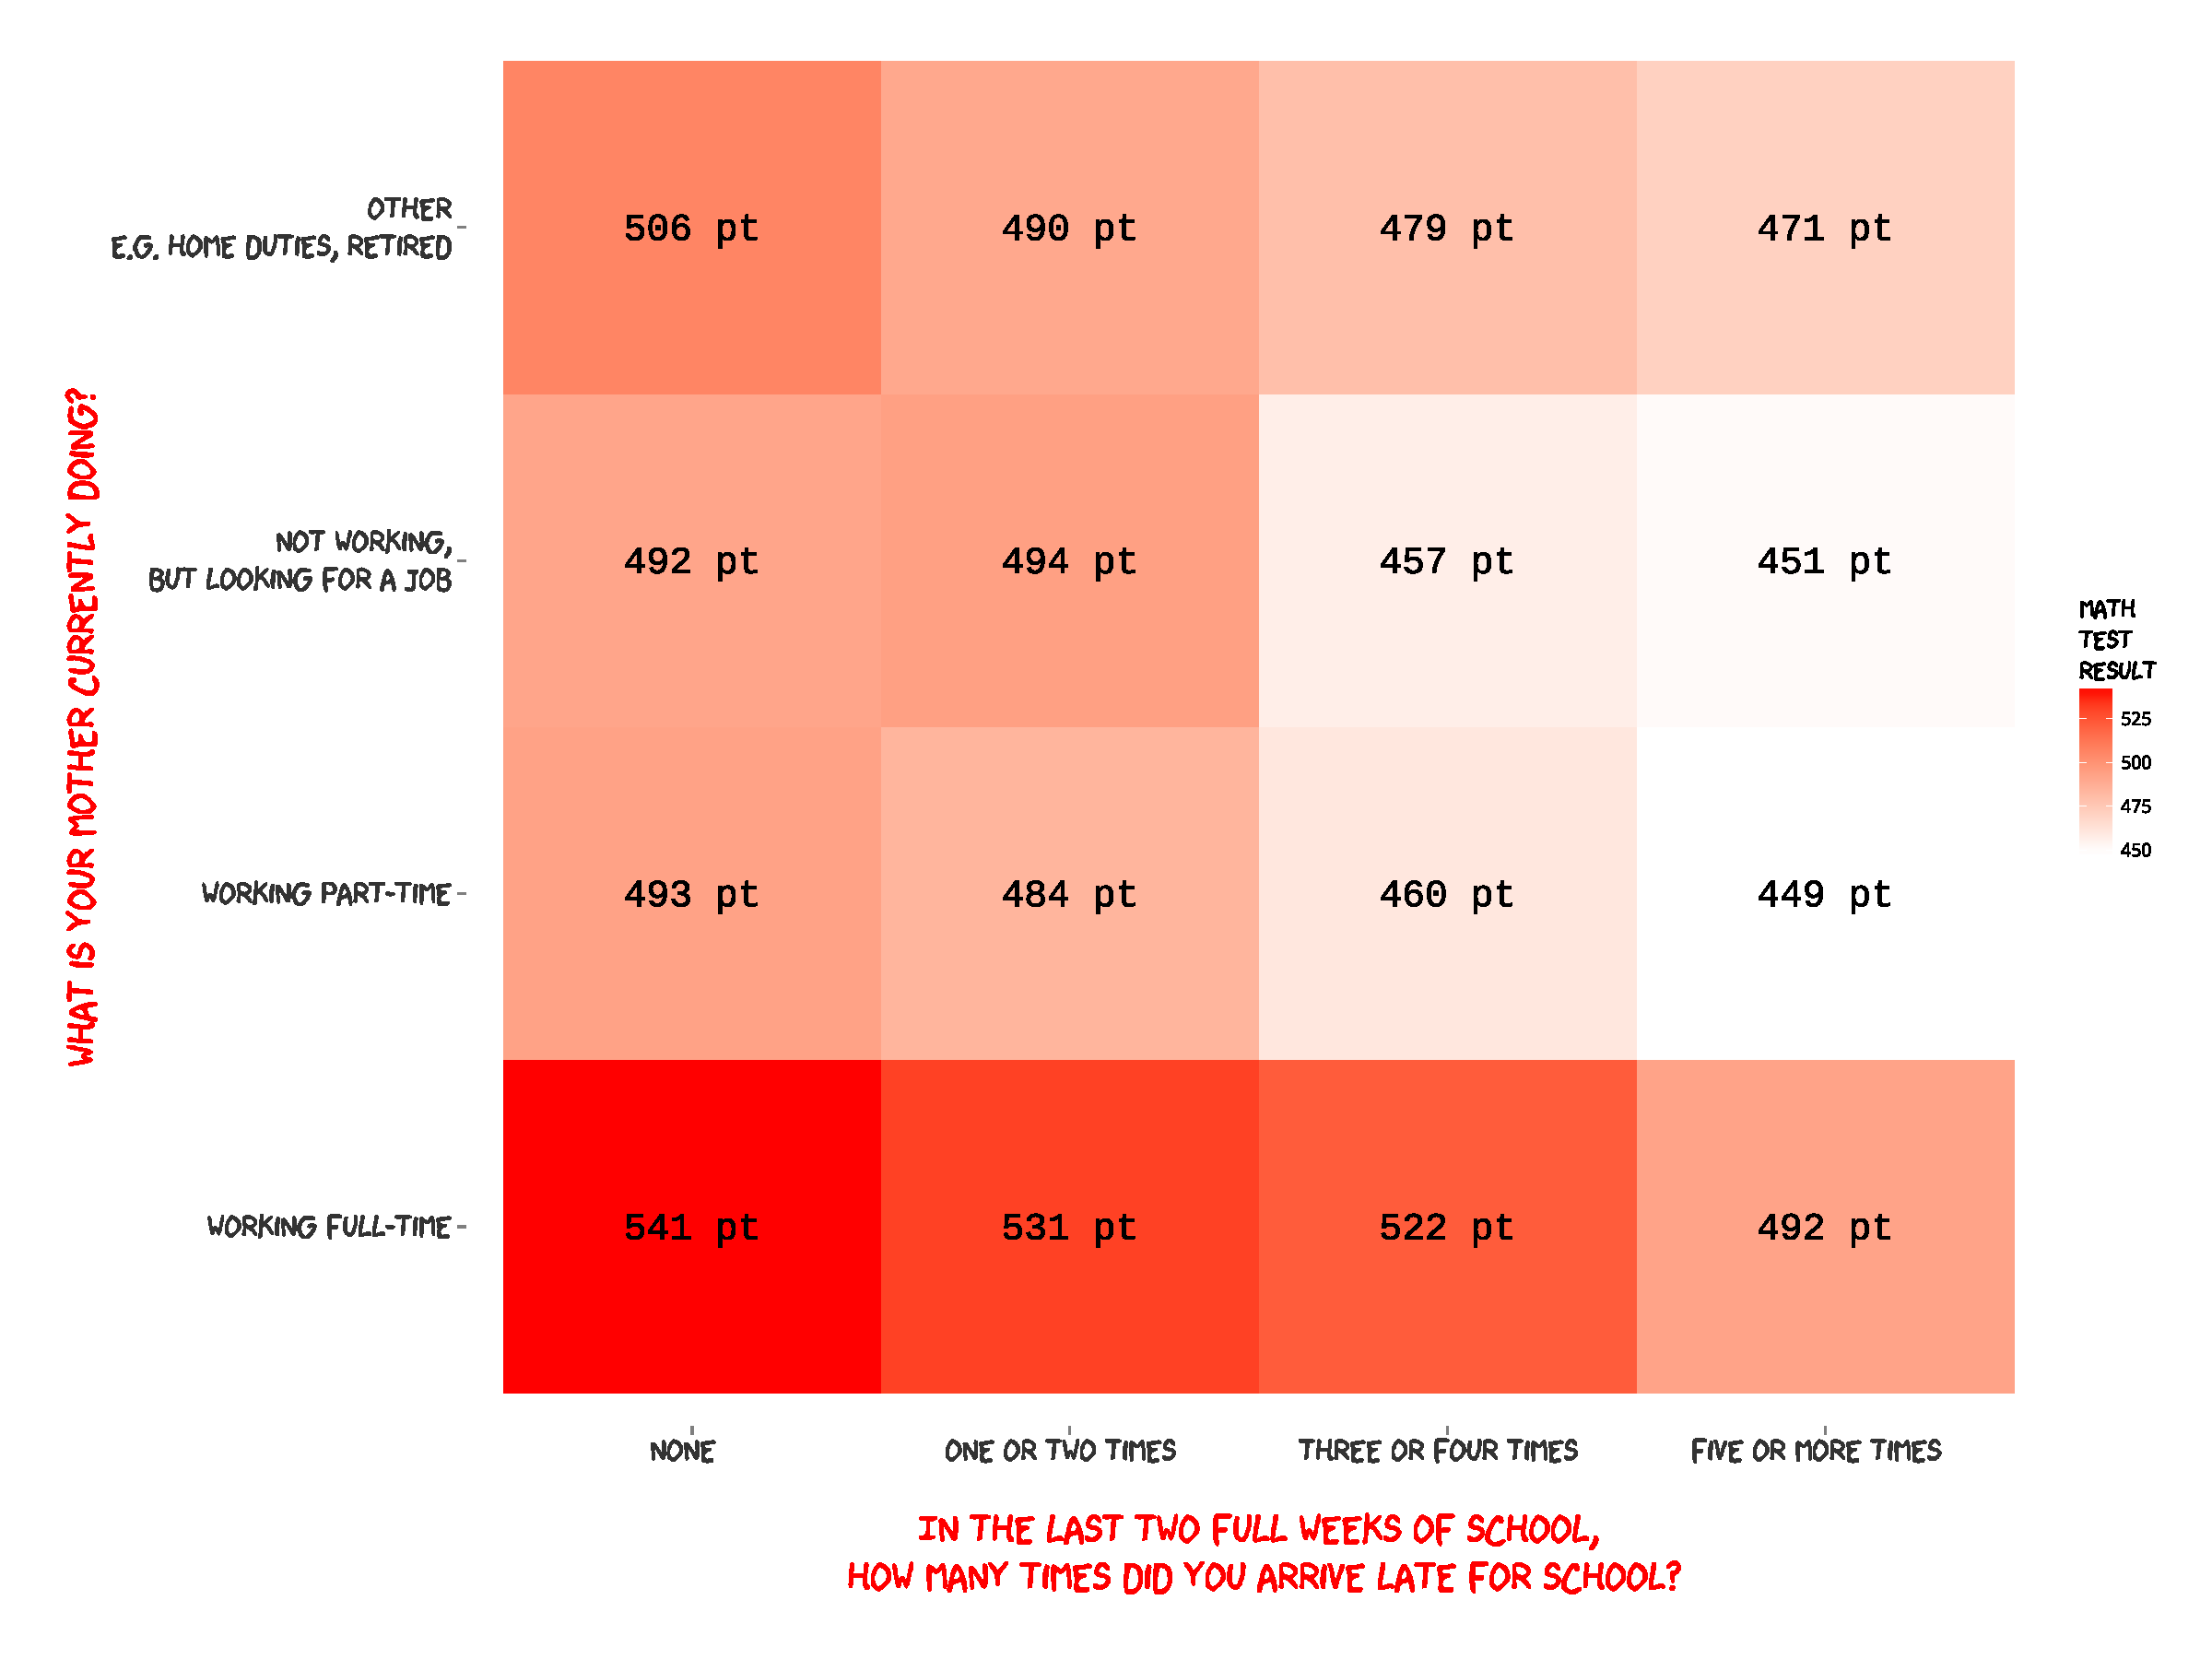
\includegraphics[width=0.9\textwidth]{graphs/Marta11.pdf}}
\blocknode{Teachers Works With Enthusiasm}{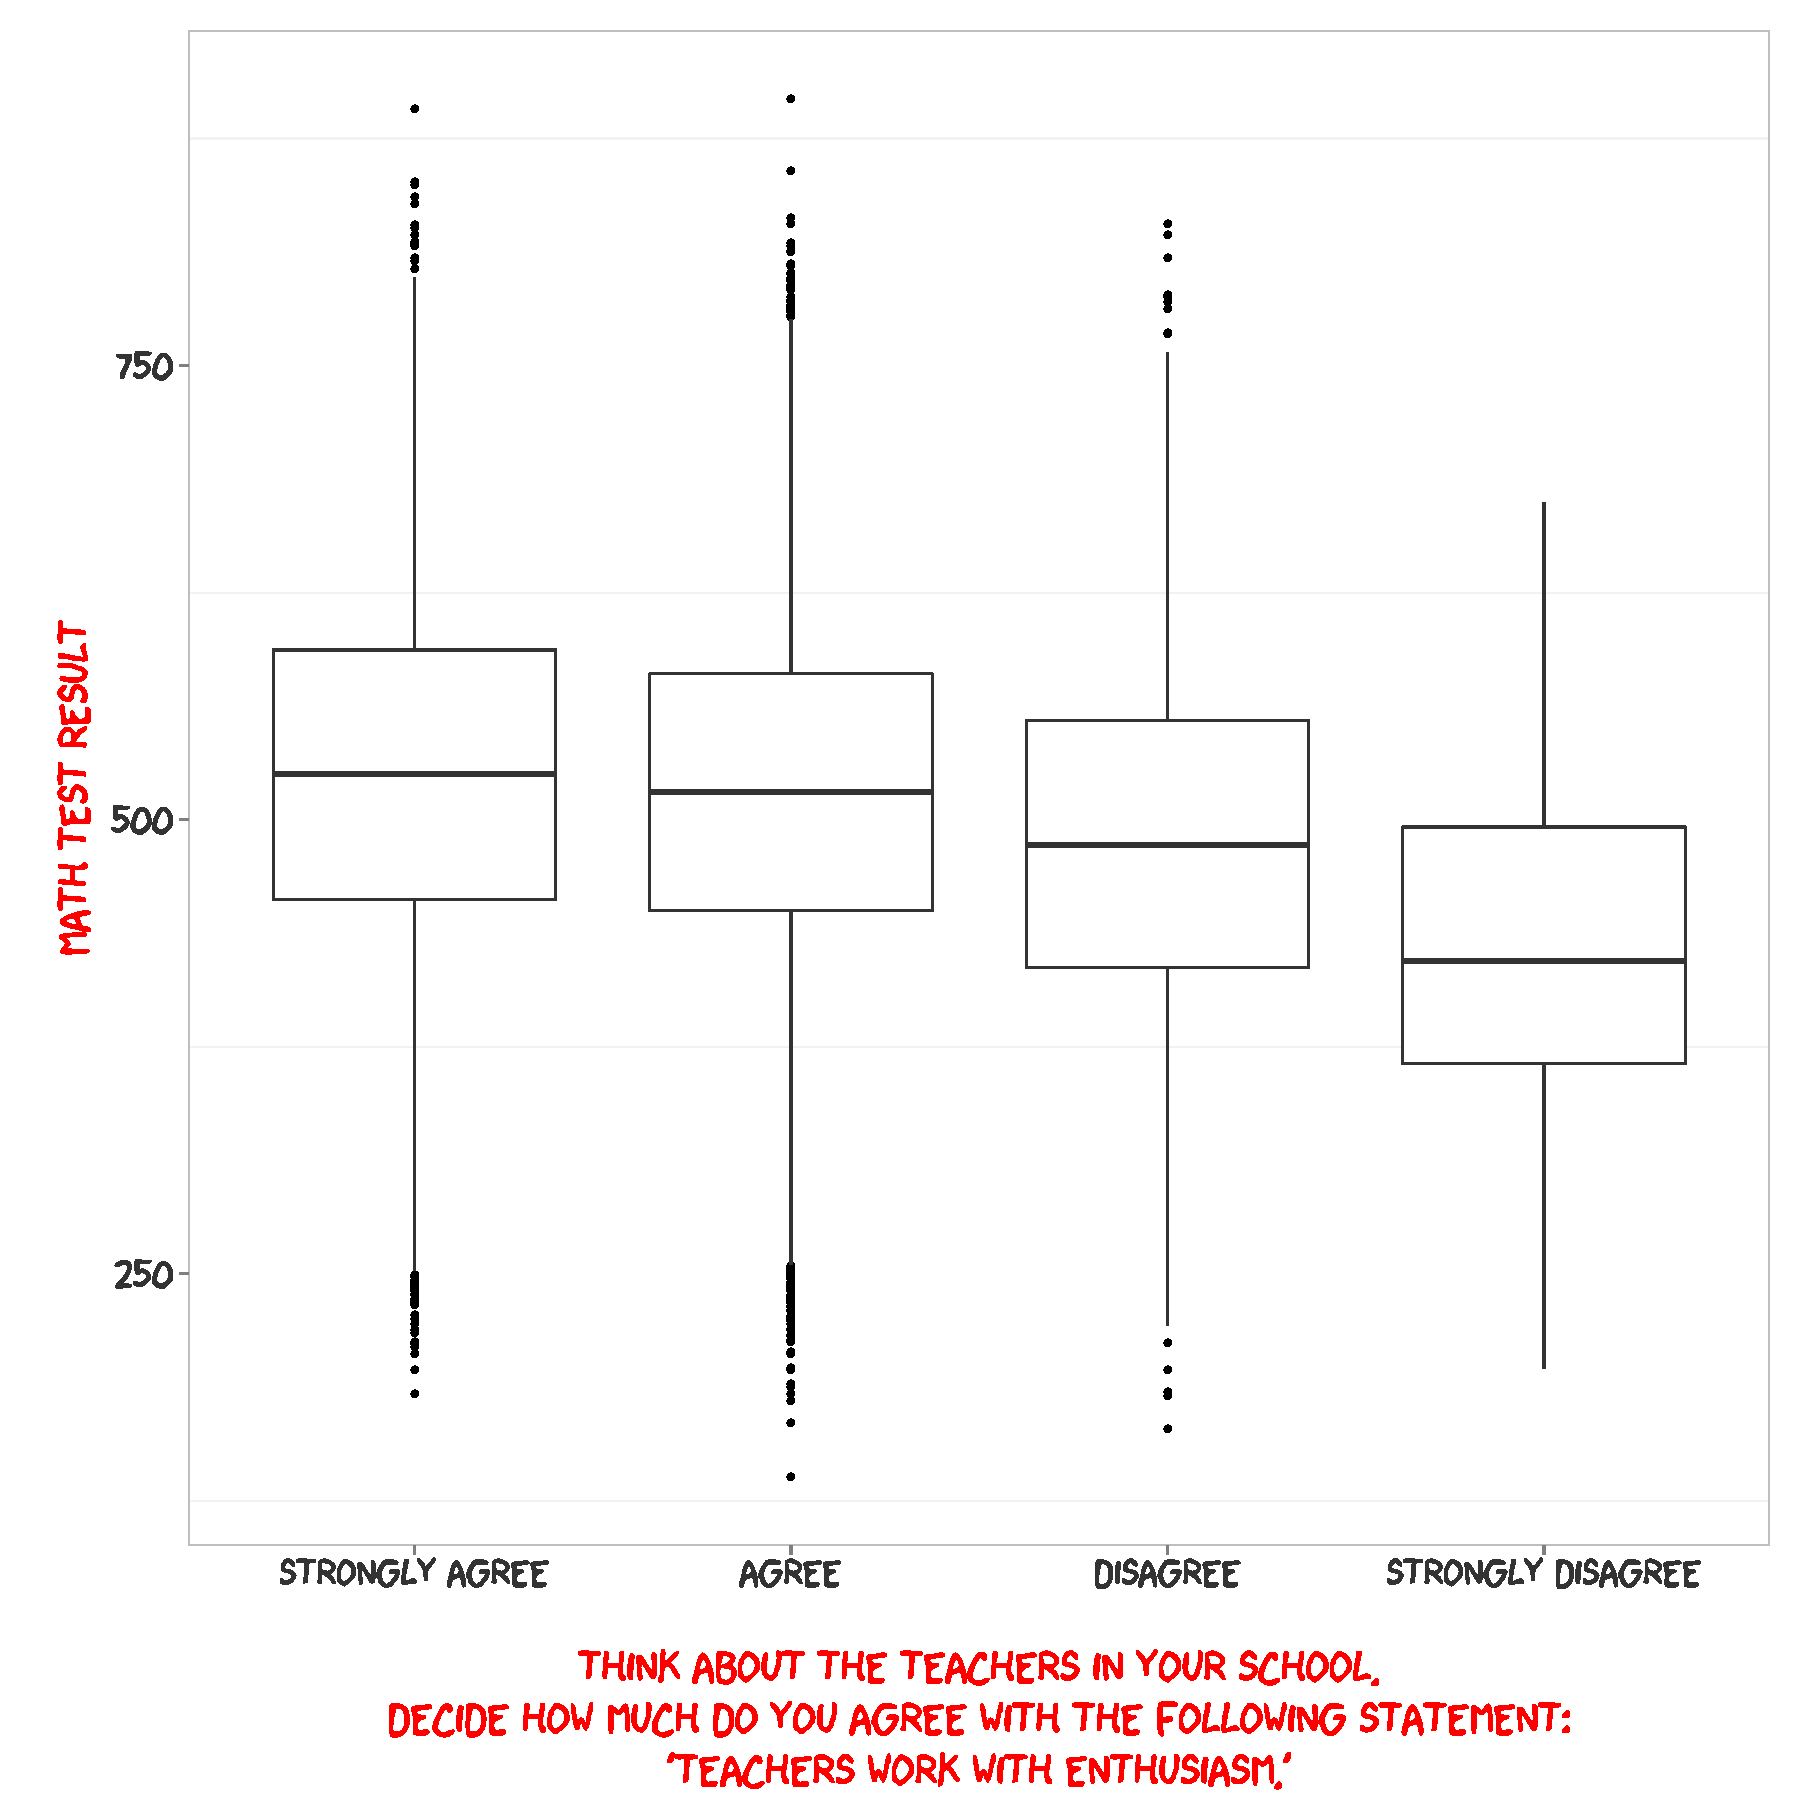
\includegraphics[width=0.9\textwidth, height=20cm]{graphs/Marta22.pdf}}
\blocknode{Final Mix}{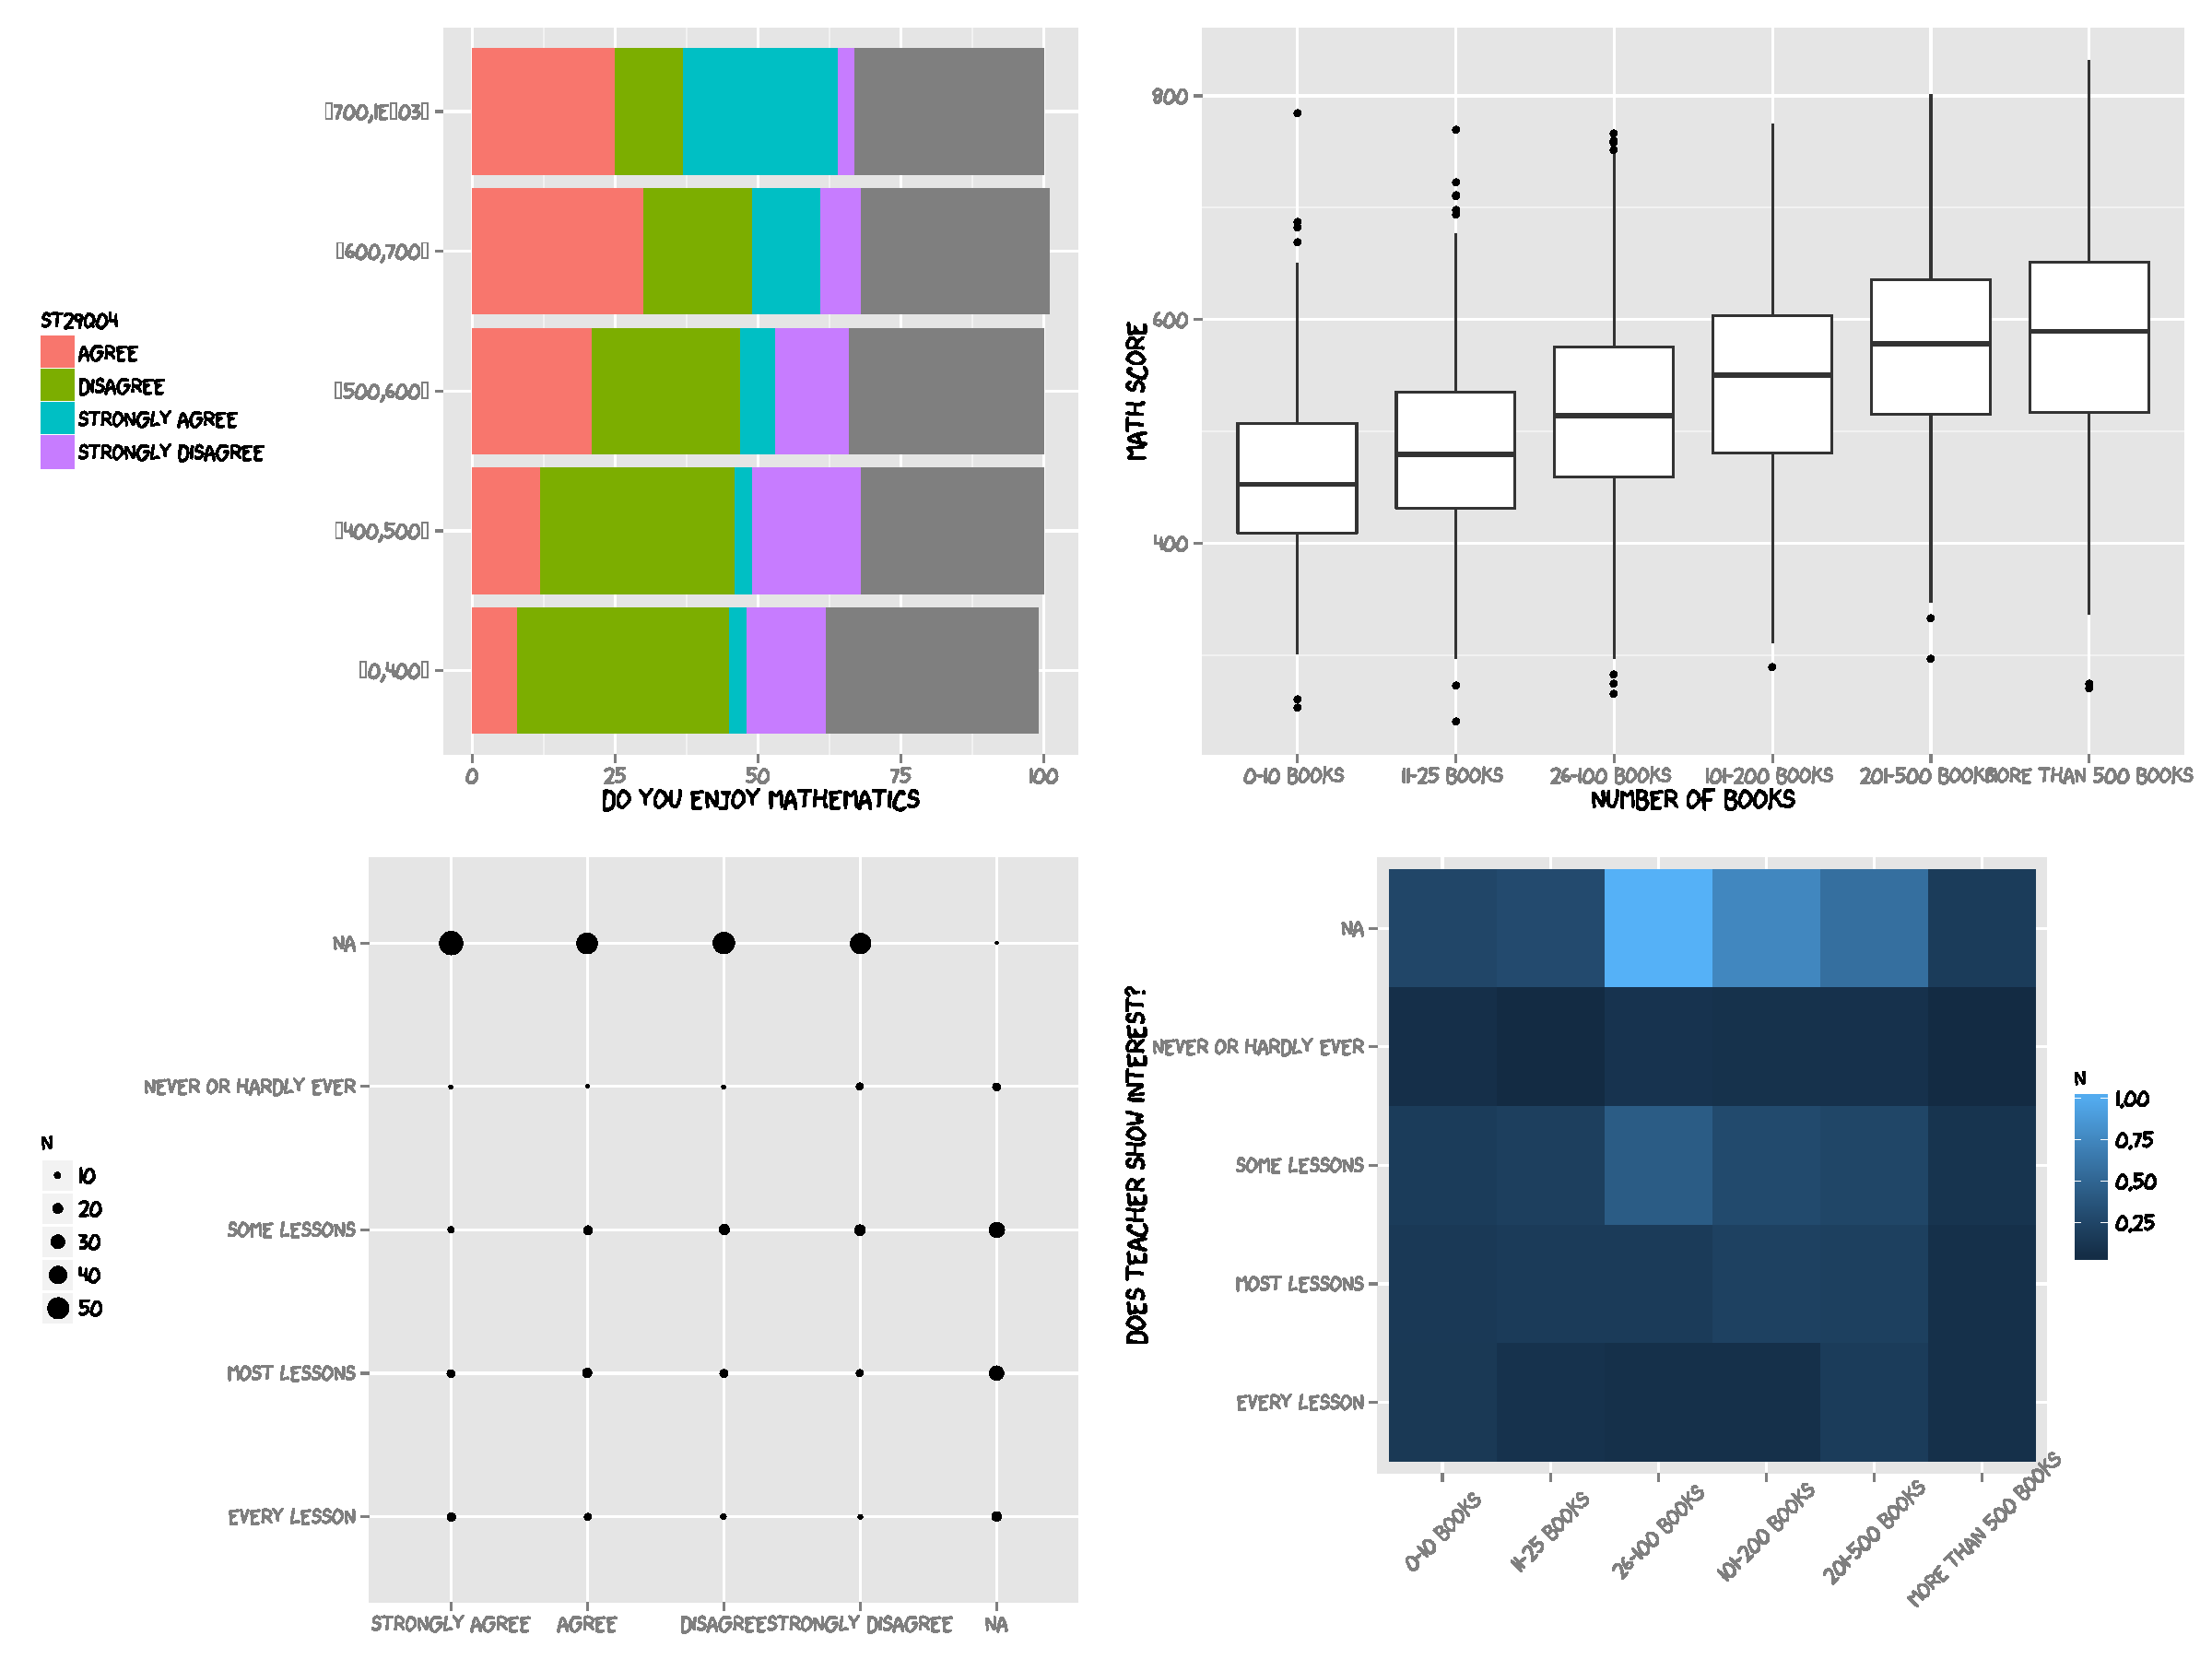
\includegraphics[width=0.9\textwidth]{graphs/Norbert11.pdf}}
\blocknode{Codes and Software}{ \centering \textbf{http://github.com/MarcinKosinski/PISAvis} }
\end{tikzpicture}
\end{document}